\section{Experimental Setup}
\label{sec:exp}

The main objective
is to look at the high power regime,
attractive for intra-cavity frequency mixing.
For this,
I report on the light-light performance
of $1270\,\mathrm{nm}$ waveband VECSELs
with wafer fused gain mirrors
set in the flip-chip heat dissipation scheme,
see section~\ref{sec:basics}.
The light-light characteristics
relates the pumped input power
with the converted
emission power.
is recorded for various heat sink temperatures.
To asses the thermal management
we determine the thermal resistance
of our device.
Following section \ref{sec:rth},
we have to keep track of
the pumped,
reflected,
and emitted power,
and the emitted spectra.

\subsection{Setup and sample}
\label{sec:exp:setup}

\begin{figure}
\centering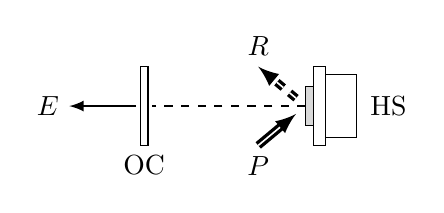
\begin{tikzpicture}[>=latex]
    %%%%%%%%%%%%%%%%%%%%%%%%%%%%
    % requires libraries:
    % \usetikzlibrary{arrows,decorations.pathmorphing,backgrounds}
    %%%%%%%%%%%%%%%%%%%%%%%%%%%%
    \begin{scope}[xshift=0cm]
    % sample holder
    \draw (0.25,0.1) rectangle (0.65,.9);
    \node[right] at (0.7,0.5) {HS};
    \draw (0.1,0) rectangle (0.25,1);
    \filldraw[fill=gray!30] (0,0.25) rectangle (0.1,0.75);

    % pump
    \draw[->,very thick,double] (-0.6,0) -- (-0.12,0.4)
        node[pos=0,below] {$P$};
    \draw[->,very thick, double, dashed] (-0.12,0.6) -- (-0.6,1)
        node[pos=1,above] {$R$};

    %laser
    \draw[thick,dashed] (0,0.5) -- (-1.95,0.5);
    \draw[->,thick] (-2.15,0.5) -- (-3,0.5)
        node[pos=1,left] {$E$};

    \draw (-2,0) rectangle (-2.1,1);
    \node[below] at (-2.05,0) {OC};
    \end{scope}

\end{tikzpicture}

\caption{The sample is mounted on a
water cooled heat sink (HS).
The external cavity is defined by the output coupler (OC)
and the active mirror
attached to the HS.
The pump is incident at
approximately $36\,^\circ$, with power $P$.
We are further interested in
the emitted power $E$,
and the reflected power $R$.}
\label{img:setup_sketch}
\end{figure}

Figure~\ref{img:setup_sketch} depicts
the basic scheme of the used setup:
The VECSEL sample is mounted
on a water cooled heat sink,
and is optically pumped by power $P$,
with a pump spot size
of radius $w$.
Some of this pump light is
converted and emitted ($E$),
reflected off the sample ($R$),
and the rest is said to be dissipated ($D$),
through the sample
onto the heat sink.
For the light-light characteristics
we are interested
in the relation between $P$ and $E$.
Respectively,
we are interested in
how much of the net pump light
is converted into emitted light.
This net pump we signify as
absorbed power
\begin{equation}
A = P-R.
\label{eq:abspwr}
\end{equation}
This definition
of absorbed power
overestimates
the real absorbed power,
it ignores
surface scattering and
spontaneous emission outside the cavity.
For the experiments
presented this report,
I ignore these loss channels.

The pump is a $980\,\mathrm{nm}$ diode laser.
Figure~\ref{img:pumpspectrum} illustrates the spectrum
for two different pump currents.
The pump is delivered by a multimode fiber.
We image its end onto the sample,
under an incidence angle
of approximately $36\,^\circ$,
using various lenses.
This results in
the various spot diameters
$2w=\{180,200,300,333,400,444\}\,\mu\mathrm{m}$.
To ensure good mode overlap
the cavity lengths has to be adjusted.

\begin{figure}
\centering
\subfigure{\includegraphics[width=7cm]{img/PumpSpectrum30p3A.png}}
\subfigure{\includegraphics[width=7cm]{img/PumpSpectrum74p9A.png}}
\caption{Spectrum of nominally $980\,\mathrm{nm}$ pump beam;
measured at $\approx6\,\mathrm{cm}$ distance to
divergent pump delivery fiber,
under $0\,^\circ$ incidence.
The plots correspond to an optical output of
$21\,\mathrm{W}$ and $56\,\mathrm{W}$,
respectively.}
\label{img:pumpspectrum}
\end{figure}

The VECSEL-sample is designed to emit
around $1270\,\mathrm{nm}$.
The fabrication details are published elsewhere
\cite{Ranta2014OptLett,Sirbu2014SPIE};
they are not part of this report.
The essential details are highlighted
in section~\ref{sec:basics},
section~\ref{sec:intro}.

Monitoring the reflection
off the sample
is crucial for high power operation.
For one,
we want to design the VECSEL structure
such that it absorbs as much
of the pump light as possible.
Secondly, depending on the exact application
the VECSEL is used for,
the reflected light may pose
a health hazard;
or at least an additional heat spot
that needs to be taken care of.

The thermal resistance $\Rth$
connects the sample temperature
with the dissipated power (\ref{eq:rth})
\begin{equation}
T = \Rth D.
\end{equation}
The performance of a VECSEL depends on temperature.
The thermal management of the device is thus critical
\cite{Tropper2006,Kemp2008,Vetter2012}
and thus a low thermal resistance is desired.
Furthermore,
the thermal resistance
is the only experimentally accessible quantity
to assess the heat flow in a VECSEL \cite{Heinen2012}.
Beside the quantities mentioned in Fig.~\ref{img:setup_sketch},
in order to estimate the thermal resistance
we also need to record the spectrum of the emitted light
\cite{Ranta2014OptLett,Heinen2012},
see section~\ref{sec:rth}.

Figure~\ref{img:setup_photo} shows a photograph of our setup.
It meets the specifications
to measure pumped,
reflected, and
emitted power,
as well as the spectra
simultaneously.
The pumped and reflected power
we measure by sampling
a fraction of the beam.
The reflectivity of these beam sampler
depend on the incidence angle.
This beam sampling fraction
needs thus to be recalibrated
whenever we change the beam sampler configuration.
We have to adjust the configuration
for example when we change
the pump spot size.

The pump spot size we vary
by changing the lenses
used to image the fiber end
onto the sample.
In Fig.~\ref{img:setup_photo}
these are denoted as
$\mathrm{L}_\mathrm{p1}$ and $\mathrm{L}_\mathrm{p2}$.
The distance between delivery fiber
and the first lens has to
correspond to its focal length.
In this configuration
the beam after the first lens is collimated.
This arrangement we test by eye,
with the help of an IR-viewer.
The pump spot is at
a distance of a focal length
after the second lens.

In order to find the exact distance,
we look for the alignment
with the lowest lasing threshold --
visualized by a camera
in the emission path.
This initial position
is further optimized
during the fine-alignment
of the output coupler,
aiming at optimal output power.
 
The ratio in focal lengths
of the two employed lenses
corresponds to obtained spot size.
I report the usage
of two types of lenses
for lens $\mathrm{L}_\mathrm{p1}$:
a plano-convex,
spherical lens
motivated by the publications
by Heinen et al. \cite{Heinen2012el,Heinen2012};
and a plano-convex, achromatic lens.
Given the fairly narrow pump spectrum
depicted in Fig.~\ref{img:pumpspectrum}
we wouldn't expect
the achromaticity itself
to have much of an effect.
On the other hand,
the achromatic doublet
has been corrected
for various aberrations \cite{ThorlabsAC}.
This may contribute
a relevant beam property.
All lenses,
as well as the beam samplers,
are appropriately coated
(meaning B- and C-coated
in the pump and emission branch,
respectively).

\begin{figure}
\centering
\includegraphics[width=14.5cm]{img/setup_photo.png}
\caption{The pump light is delivered
with a $200\,\mu\mathrm{m}$ multimode (MM) fiber
whose end is imaged onto the sample.
The sample is
mounted on a water cooled copper heat sink.
We image
using various lenses
($\mathrm{L}_\mathrm{p1}$,$\mathrm{L}_\mathrm{p2}$),
resulting in various spot sizes.
The reflected, divergent light
is collected by lens $\mathrm{L}_\mathrm{r}$
and subsequently directed onto a beam dump.
The two beam sampler
($\mathrm{BS}_\mathrm{p}$ and $\mathrm{BS}_\mathrm{r}$)
probe a fraction of the pumped
and reflected light.
This beam sample is directed
to their respective detectors
($\mathrm{D}_\mathrm{p}$ and $\mathrm{D}_\mathrm{r}$).
The sample,
together with the output coupler (OC),
form the external cavity.
The OC has an output coupling loss
$\alpha_\mathrm{OC}=2.5\,\%$,
and a radius of curvature
$ROC=50\,\mathrm{mm}$.
The VECSEL emission
is collected by lens $\mathrm{L}_\mathrm{e}$
and directed onto power meter $\mathrm{D}_\mathrm{e}$.
A fraction of this output
is extracted by beam sampler $\mathrm{BS}_\mathrm{e}$
and directed onto the MM-fiber
connected with the optical spectrum analyzer (OSA).
The polarization
of neither
pump nor emission
is filtered,
in our setup
we do not distinguish
between polarization dependent phenomena.
Cameras 1 and 2 facilitate the alignment.}
\label{img:setup_photo}
\end{figure}

The sample is attached on a ceramic plate,
which itself is attached
to a water cooled copper block,
using thermal grease.
The reported heat sink temperature
is the temperature we measure
at the copper block.
Due to the irradiated power
the heat sink cannot keep a constant temperature.
As a result the measurements
see a fluctuation of about
$\pm$\degr{1} standard deviation.
These temperature fluctuations are addressed
again in subsection~\ref{sec:exp:measroutine}.

I have worked with
two samples,
addressing a proposed optimization strategy
\cite{Hader2011}.
A magnified photo of
sample 1 is shown in Fig.~\ref{img:sample_surface}.
It is illuminated by $980\,\mathrm{nm}$ pump light,
highlighting the defects
that don't contribute to photo luminescence.
The camera has burnt spots itself.
In order not to confuse
the camera defects
with those of the structure,
I have covered those of the camera
with blue dots.
The presented measurements
were taken when irradiating
either of the two regions
denoted as A and B,
respectively.

We investigate the effect
of two optimization strategies
\cite{Hader2011}.
First, we have coated this same sample 1
with an anti-reflection coating.
The surface integrity
after the necessary
surface treatment
and coating
is shown in Fig.~\ref{img:sampleAR_surface}.
It doesn't highlight the surface roughness
which visibly worsened
because of the coating.
This lead to poorer performance,
as will be discussed
in section~\ref{sec:eval:maxout}.

For the second optimization
the gold layer between the DBR
and the CVD diamond
is treated to be highly reflective.
For this measure
we have to take a second sample.
Its active region and DBR
are identical
with those of sample 1.
Figure~\ref{img:sampled6_surface}
shows the surface integrity
of sample 2.

\begin{figure}
\centering
\includegraphics[width=6cm]{img/sample_surface.png}
\caption{Sample 1.
Used for pump spot scaling.
Magnified by a microscope,
illuminated with $980\,\mathrm{nm}$ light.
This light source makes visible
the defects of the structure;
as the dark spots will also be dark
when pumped during laser operation.
The blue dots cover defects
of the used camera,
which otherwise may be mistaken
as defects of the sample.
The red circles indicate
irradiation region A and B,
respectively.
The sample dimensions are $3\times3\,\mathrm{mm}$.}
\label{img:sample_surface}
\end{figure}

\begin{figure}
\centering
\includegraphics[width=6cm]{img/sampleAR_surface.png}
\caption{Sample 1 from Fig.~\ref{img:sample_surface},
after surface treatment and AR coating.
The brightness cannot be compared
with the one from Fig.~\ref{img:sample_surface},
the camera is not calibrated for such a comparison.
The illumination at $980\,\mathrm{nm}$
shows non-radiative defects,
but it doesn't show the surface roughness.
The red circle indicates the tested spot.}
\label{img:sampleAR_surface}
\end{figure}

\begin{figure}
\centering
\includegraphics[width=6cm]{img/sampled6_surface.png}
\caption{Sample 2.
Used to investigate
an optimization strategy:
reflecting metalization layer behind the DBR.
The brightness cannot be compared
with the one from Fig.~\ref{img:sample_surface},
the camera is not calibrated for such a comparison.
The $980\,\mathrm{nm}$ light source
makes visible
the non radiative defects of the structure.
The blue dots cover camera defects.
The red circles indicates
the tested spot.
The sample dimensions are $3\times3\,\mathrm{mm}$.}
\label{img:sampled6_surface}
\end{figure}

\subsection{Measurement routine and error bars}
\label{sec:exp:measroutine}

For each light-light characteristic
we vary the incident pump power $P$
and the temperature of the heat sink $\Ths$.
The varying heat sink temperature
is required to determine
the thermal resistance,
see section~\ref{sec:rth}.

The heat sink temperatures are partially set
in ascending and descending order, Fig.~\ref{img:temp_order}.
This allows us to save time,
since the heat reservoir
providing the temperature stabilized water
is inert.
On the other hand,
this routine also indicates
whether the results are consistent
or depend on the temperature cycle
they were measured in.
And last but not least,
this routine allows us
to see whether or not
the sample takes damage
as a result of the elevated temperature;
a property vital for real world applications.

\begin{figure}
\centering
\includegraphics[width=6cm]{img/temp_order.png}
\caption{An example for the temperature order.
Some of the temperatures
are set
while heating up,
the rest while cooling down.
The objective is to save time,
to have a consistency check,
and to see whether the sample
shows fatigue after heating it up.}
\label{img:temp_order}
\end{figure}

At each heat sink temperature
we irradiate the sample
with different pump powers.
Each pump is repeated $N$ times over all.
The pump order is selected at random,
as illustrated in Fig.~\ref{img:random_sampling}.
Thanks to the random sampling
the measurement results
are detached from the lab environment --
most notably time-independent.
The heat sink cannot control its temperature
with absolute precision.
Figure~\ref{img:random_sampling_heatsink}
illustrates this issue:
It shows
the actually present heat sink temperature
for six set temperatures.
In the left column
the temperatures are plotted
in chronological order.
We can identify,
the temperature drifts.
The right column shows the same temperatures,
but corresponding to the set pump.
The repeated measurements
see a spread of different temperatures
but the temporal drifts can not be resolved.

In contrast,
Fig.~\ref{img:random_sampling_ramp_heatsink}
shows the heat sink temperature
during a measurement without the random pump selection.
In this case, clearly,
we cannot talk about a single heat sink temperature
for all the pump settings
for this specific set heat sink temperature.
The resulting measurements are highly repeatable,
but only given the same pump order.
This pseudo-stability
we exploit
during the calibration process
of the different beam samplers
and detectors:
During the calibration
we don't care about reproducibility
but solely about the repeatability
of two consecutive measurements.

\begin{figure}
\centering
\subfigure{\includegraphics[width=7cm]{img/random_sampling_ramp.png}}
\subfigure{\includegraphics[width=7cm]{img/random_sampling_random.png}}
\caption{Two examples to apply various pump settings, with a repetition rate of 3.
Left: A ramp. Right: Random sampling.}
\label{img:random_sampling}
\end{figure}

\begin{figure}
\centering
\includegraphics[width=15cm]{img/random_sampling_heatsink.png}
\caption{The heat sink temperature fluctuates over time (left).
Thanks to the random sampling addressed in Fig.~\ref{img:random_sampling}
the measurements don't see these drifts (right).}
\label{img:random_sampling_heatsink}
\end{figure}

\begin{figure}
\centering
\subfigure{\includegraphics[width=7cm]{img/random_sampling_ramp_heatsink.png}}
\subfigure{\includegraphics[width=7cm]{img/random_sampling_ramp_noisfreeLL.png}}
\caption{In contrast to Fig.~\ref{img:random_sampling_heatsink},
when we ignore the random pump sampling
highlighted in Fig.~\ref{img:random_sampling},
the temperature seen by the single pump settings
differ strongly from the average heat sink temperature
(left).
The resulting LL-characteristic
has very little noise on its data points
(right).
But these small error bars dismiss the fact
that the underlying points were measured
under very different conditions;
eroding the significance
of this low noise.}
\label{img:random_sampling_ramp_heatsink}
\end{figure}

The power meter average each measurement point
over 200 samples,
of which each one sample
takes approx. 3 ms \cite{ThorlabsPM}.

As mentioned already,
we repeated the measurement of each pump setting
$N$ times.
With this repetition we obtain a measure
for how well we know
the underlying true value.
We are hence interested in
the mean of these single measurements and
the resulting unbiased standard error \cite{Barlow}
\begin{equation}
\Delta x = \sqrt{ \frac{1}{N(N-1)}
	\sum\limits_{i=1}^N (x_i - 
		\frac{1}{N} \sum\limits_{i=1}^N x_i )^2 }.
\label{eq:sterr}
\end{equation}

For the uncertainties attached to
quantities obtained through fits,
I use a so-called
Jackknife \cite{Efron1983} approach:
In a nutshell,
this method allows to estimate
the influence of the single measurement points
on the fit parameters
without working through
the covariance matrix of the fit.
The resulting error value
is directly related with the
unbiased standard error (\ref{eq:sterr}),
used for the rest of the report.

